
\section{Обзор предметной области}

\subsection{Обзор аналогов разрабатываемого продукта}
Разрабатываемый продукт представляет собой прототип образовательного робототехнического комплекта на базе БПЛА.

Из существующих на российском рынке решений можно выделить нес\-колько наборов, базой -- носителем каждого из которых является БПЛА мультироторной схемы типа квадрокоптер:

1. Набор Copter Express <<Клевер>>.

Технические характеристики:
\begin{itemize}
	\item размер 330*330 мм;
	\item диаметр винтов 5" (дюймов);
	\item вес порядка 600 г;
	\item карбоновая рама;
	\item литий-полимерный аккумулятор напряжением 16.8 В объемом 2300 мАч;
	\item электроника своего бренда.
\end{itemize}

Функциональные возможности включают полет в режиме ручного управления и автономный полет по полю меток при помощи бортовой камеры и одноплатного бортового компьютера Raspberry Pi (RPi), на котором выполняются все вычисления. Стоимость комплекта от 79 тыс. руб.. Существенным недостатком данного варианта является его большие размер и мощность, что делает его использование травмоопасным. При использовании данного комплекта необходимо отдельное помещение и огороженная сеткой территория внутри него. Также стоимость нескольких таких комплектов в некоторых случаях превышает бюджет образовательных организаций.

2. Геоскан <<Пионер Мини>>.

По сравнению с предыдущим аналогом комплект <<Пионер Мини>> обладает маленьким размером (130 мм диагональ рамы). На борту установлена плата собственной разработки с размещенными на ней полетным контроллером, регуляторами, радиоприемником и коннекторами для подключения моторов. Цена дрона от 14 тыс. руб.. Минусом данного набора является то, что для решения задачи позиционирования помимо комплекта дрона необходимо приобрести отдельно систему навигации в помещении, цена которой начинается от 58 тыс. руб., и, в отличии от <<Клевера>>, проект не развивается с 2019 года.

3. MiniBot <<Nanopix>>.

Nanopix представляет собой квадрокоптер на коллекторных моторах размером 80 мм по диагонали, стоимость базового комплекта от 8 тыс. руб.. Рама напечатана пластиком, имеется защита пропеллеров. Такой комплект отлично подходит для начальных классов. Возможно программирование на Scratch, Arduino или Python через Wi-Fi. Ключевым недостатком Nanopix является базирование на платформе Arduino, из-за чего вычислительных мощностей хватает только для самых простых задач.

4. BRLAB <<EDU.ARD мини>>

Это довольно новый продукт, ввиду чего малоизвестен. По габаритам схож с комплектом от Геоскан, стоимость от 11 тыс. руб.. На борту стоит электроника собственного производства, имеется подробная документация по настройке и эксплуатации дрона. Комплект подходит для школ и учреждений дополнительного образования для изучения базового уровня программирования и управления БПЛА, однако невозможно использование компьютерного зрения, ввиду чего возможности автономного полета ограничены.

На рисунке \ref{fig:ris0} представлены дроны из упомянутых комплектов.
% ~\ref{fig:ris1}
\begin{figure}[H]
	\centering
	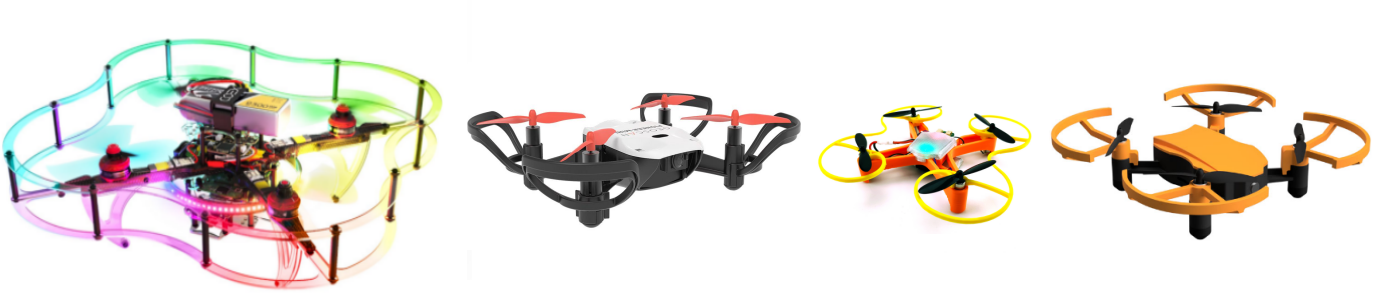
\includegraphics[width=0.8\linewidth]{./pics/analogi}
	\caption{Аналоги разрабатываемого продукта
	}
	\label{fig:ris0}
\end{figure}

\subsection{Математическая модель квадрокоптера}

Для понимания принципов полета квадрокоптера рассмотрим его математическую модель в двух системах координат (СК):

1. Неподвижная система координат (НСК), в качестве которой выступает нормальная земная система координат с заданными перпендикулярными друг другу координатными осями \(O_{g}X_{g}\), \(O_{g}Y_{g}\), и \(O_{g}Z_{g}\), причем ось \(O_{g}Z_{g}\) направлена противоположно вектору силы тяжести.

2. Связанная с квадрокоптером система координат (ССК), центр которой размещен в центре масс аппарата, а оси \(OX\), \(OY\), и \(OZ\) параллельны и сонаправлены с осями неподвижной системы. Угловое положение аппарата зададим тремя углами Эйлера: углами крена \(\phi\), тангажа \(\theta\) и рыскания \(\psi\), определяющими вращение вокруг осей \(OX\), \(OY\), и \(OZ\) соответственно. Основываясь на ранее рассмотренных системах координат можно утверждать о том, что квадрокоптер имеет шесть степеней свободы, а именно три линейных координаты \([x; y; z ]\) и три угловых \([\theta, \phi, \psi]\). В качестве управляющих каналов выступают скорости вращения роторов (рисунок \ref{fig:ris1}), которые создают динамику движения БПЛА в пространстве. Возникающие в результате подачи управляющих воздействий силы и моменты пропорциональны квадрату угловых скоростей винтов \(\Omega^2\). Поэтому, для достижения желаемого режима работы БПЛА, необходимо связать совокупность управляющих воздействий со степенями свободы БПЛА, через уравнения связи, которые определяют основные режимы движения квадрокоптера в пространстве.
% ~\ref{fig:ris1}
\begin{figure}[H]
	\centering
	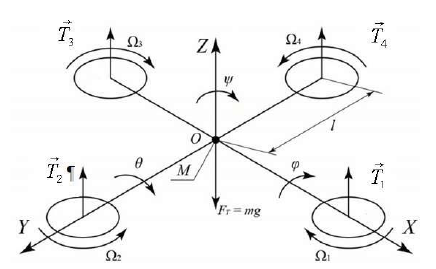
\includegraphics[width=0.5\linewidth]{../RW/pics/ris1}
	\caption{Связанная система координат квадрокоптера
	}
	\label{fig:ris1}
\end{figure}

В качестве первого режима БПЛА \(U_{1}\) рассмотрим движение вдоль оси \(OZ\), принадлежащей ССК. Данное движение обеспечивается одновременным увеличением скоростей винтов на одинаковое значение угловой скорости \(\Delta a\). Полученное при этом движение характеризуется взлетом или посадкой квадрокоптера (при нулевых значениях тангажа и крена) и описывается следующим выражением:
\begin{equation}
U_{1}=b(\Omega_{1}^2+\Omega_{2}^2+\Omega_{3}^2+\Omega_{4}^2)
\end{equation}

где \(b\) -- аэродинамическая составляющая тяги винта.
В качестве второго режима движения БПЛА \(U_{2}\) необходимо взять поворот вокруг оси \(OX\), принадлежащей ССК. Данное движение достигается путем увеличения/уменьшения на величину \(\Delta a\) значения \(\Omega_{4}\) левого винта и уменьшением/увеличением на величину \(\Delta b\) значения \(\Omega_{1}\)
правого. Полученное при этом движение характеризуется изменением угла крена \(\phi\) и описывается следующим выражением:
\begin{equation}
U_{2}=lb(-\Omega_{2}^2-\Omega_{4}^2)
\end{equation}

где \(l\) -- расстояние между центром квадрокоптера и центром винта.

В качестве третьего режима движения \(U_{3}\) необходимо взять поворот БПЛА вокруг оси \(OY\), принадлежащей ССК. Данное движение достигается путем уменьшения / увеличения на величину \(\Delta a\) значения \(\Omega_{1}\) фронтального винта и увеличения / уменьшения на величину \(\Delta b\) значения \(\Omega_{3}\) заднего. Полученное при этом движение характеризуется изменением угла тангажа \(\theta\) и описывается следующим выражением:
\begin{equation}
U_{3}=lb(-\Omega_{1}^2-\Omega_{3}^2)
\end{equation}

В качестве последнего, четвертого, режима движения \(U_{4}\) необходимо взять поворот БПЛА вокруг оси \(OZ\), принадлежащей ССК. Данное движение достигается путем одновременного увеличения/уменьшения на величину \(\Delta a\) значений \(\Omega_{4}\) левого и \(\Omega_{2}\) правого винтов, а также одновременного уменьшения / увеличения на величину \(\Delta b\) значений \(\Omega_{1}\) фронтального и \(\Omega_{3}\) заднего винтов. Благодаря вращению роторов в диагонально противоположных направлениях, полученное движение характеризуется изменением угла рыскания \(\psi\) и описывается следующим выражением:
\begin{equation}
U_{4}=d(-\Omega_{1}^2+\Omega_{2}^2-\Omega_{3}^2+\Omega_{4}^2)
\end{equation}
где \(d\) -- аэродинамическая составляющая коэффициента сопротивления среды.
Введенное с учетом (1) -- (4) множество \(U\), характеризующее режимы
движения квадрокоптера, можно записать следующим образом:

\begin{equation}
U = \left\{ \begin{aligned}
U_{1}&=&b(\Omega_{1}^2+\Omega_{2}^2+\Omega_{3}^2+\Omega_{4}^2)\\
U_{2}&=&lb(-\Omega_{2}^2-\Omega_{4}^2)\\
U_{3}&=&lb(-\Omega_{1}^2-\Omega_{3}^2)\\
U_{4}&=&d(-\Omega_{1}^2+\Omega_{2}^2-\Omega_{3}^2+\Omega_{4}^2)
\end{aligned} \right.
\end{equation}

Множество \(U\) определяет связь между системой исполнительных приводов и платформой БПЛА \cite{mathmodel}.

\subsection{Устройство квадрокоптера}
Далее рассмотрим компонентную базу квадрокоптера.

Квадрокоптер -- беспилотный летательный аппарат мультироторного типа с четырьмя несущими винто -- моторными группами (далее ВМГ). Условная схема представлена на рисунке \ref{fig:pix}.
Квадрокоптер состоит из:
\begin{itemize}
	\item рамы;
	\item 4 моторов, пропеллеров (ВМГ);
	\item 4 регуляторов оборотов (далее рассматривается как часть ВМГ);
	\item полетного контроллера;
	\item аккумулятора;
	\item камеры, видеопередатчика, видеоантенны (опционально для FPV);
	\item радиоприемника (радиопередатчика, если необходима отправка телеметрии);
	\item другой периферии (например, GPS, магнитометр, дальномер, телеметрийный модуль).
\end{itemize}

 % ~\ref{fig:pix}
 \begin{figure}[H]
 	\centering
 	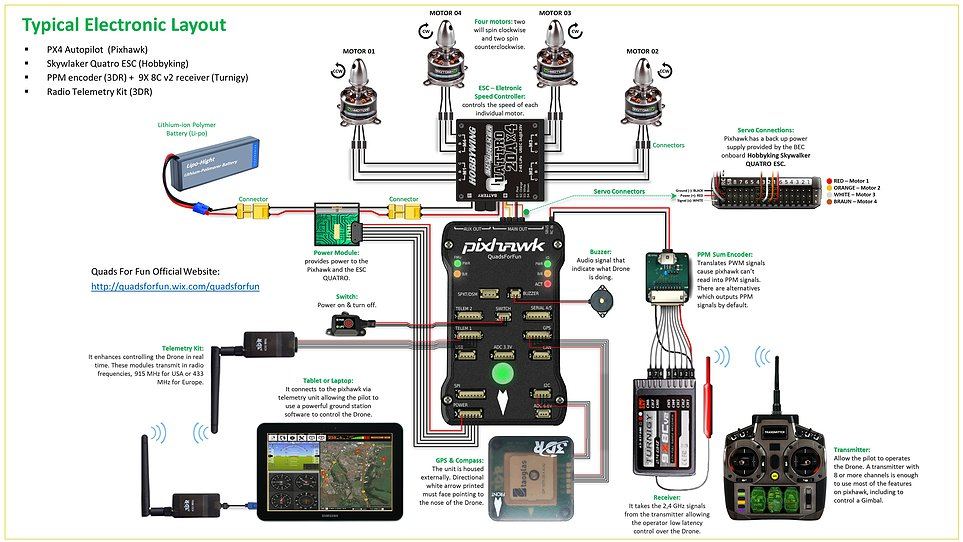
\includegraphics[width=0.5\linewidth]{../RW/pics/pix}
 	\caption{Пример схемы подключения
 	}
 	\label{fig:pix}
 \end{figure}

Рассмотрим каждый компонент с его характеристиками подробнее.

Рама -- несущий компонент, на котором располагается вся электроника квадрокоптера. Рама должна быть жесткой, прочной, и в то же время легкой. На данный момент лучшим материалом для рам квадрокоптеров является карбон.

Компоненты ВМГ подбираются в зависимости от поставленных задач и характеристик БПЛА. Для современных БПЛА используются моторы бесколлекторного типа. Основными их характеристиками являются размер и количество оборотов на вольт.
Диаметр, шаг и количество лопастей пропеллера определяют тягу квадрокоптера. При этом пропеллеры с большим шагом обеспечивают большую скорость полета.

Регулятор принимает управляющий сигнал с полетного контроллера и на его основе задает обороты моторов. В случае мотора бесколлекторного типа это происходит путем открытия силовых ключей (мосфетов) для коммутации обмоток.

Полетный контроллер -- система реального времени, которая интерпретирует входящие данные от приемника и бортовых датчиков (гироскопа, акселерометра, барометра и др.), на основе которых рассчитывает положение квадрокоптера и производит регулирование путем выдачи управляющего сигнала на ВМГ. Все алгоритмы работы полетного контроллера содержатся в прошивке -- программном обеспечении, которое выбирается в зависимости от схемы полетного контроллера и поставленных задач.

Для питания квадрокоптера используются литий-полимерные и литий-ионные аккумуляторы. В зависимости от задач и размеров подбирается количество ячеек аккумулятора, емкость и токоотдача.

Видеосистема состоит из трех основных компонентов: камера, видеопередатчик, приемник, передающая и принимающая антенны. Видеопередатчик, в большинстве случаев, функционирует на диапазоне частот 5.8 ГГц.

Для осуществления контроля над квадрокоптером используется радиоуправление. Для приема сигнала к полетному контроллеру подключается приемник, общающийся с передатчиком по определенному протоколу на указанном диапазоне частот. Информация с датчиков квадрокоптера оператору может передаваться с помощью устройств приема-передачи телеметрии.

Также на квадрокоптер возможна установка бортового компьютера для выполнения более высокоуровневых вычислительных задач, например, когда необходима обработка видеопотока или выполнение других высокоуровневых вычислительных задач прямо на борту. Как правило, бортовой компьютер представляет собой микрокомпьютер, например, Ras\-pber\-ry Pi или Nvi\-dia Jet\-son, и обмен данными между полетным контроллером и бортовым компьютером идет по проводу через usb-порт. Для дистанционного управления наиболее популярен протокол MAVLink, изучим его подробнее.

\subsection{MAVLink}
%\url{https://mavlink.io/en/}

MAVLink -- это протокол двоичной телеметрии, разработанный для систем с ограниченными ресурсами и каналов с ограниченной пропускной способностью. MAVLink был впервые выпущен в начале 2009 года Лоренцем Мейером (основателем ПО для полетных контроллеров PX4) и в настоящее время имеет значительное количество разработчиков. Протокол развернут в двух основных версиях: v1.0 и v2.0, которые имеют обратную совместимость (реализации v2.0 могут анализировать и отправлять пакеты v1.0).

MAVLink реализует гибрид шаблонов проектирования взаимодействия «публикация -- подписка» и «точка -- точка». В этом гибридном шаблоне потоки данных отправляются / публикуются как темы, а подпротоколы конфигурации, такие как протокол задания или протокол параметров, реализуются шаблоном «точка-точка» с повторной передачей.

Сообщения определяются в файлах XML. Каждый файл XML определяет набор сообщений, поддерживаемый MAVLink системой, также называемый «диалектом». Набор эталонных сообщений, который реализуется большинством наземных станций управления и автопилотов, определен в common.xml (большинство диалектов основано на этом определении).

Набор инструментов MAVLink использует определения XML сообщений для генерации библиотеки MAVLink для каждого из поддерживаемых языков программирования. Дроны, наземные станции управления и другие системы MAVLink используют сгенерированные библиотеки для связи. Они распространяются под лицензией MIT и поэтому могут использоваться без ограничений в любом приложении с закрытым исходным кодом без публикации исходного кода. MAVLink был впервые выпущен в начале 2009 года Лоренцем Мейером (основателем PX4) и в настоящее время имеет значительное количество разработчиков \cite{px}.

MAVLink поддерживает множество языков программирования, работающих на множестве микроконтроллеров / операционных систем (включая ARM7, ATMega, dsPic, STM32 и Windows, Linux, MacOS, Android и iOS). Допускает одновременно до 255 систем в сети (беспилотники, наземные станции и т. д.)

Обеспечивает как внешнюю, так и бортовую связь (например, между q\-ground\-con\-trol и дроном, а также между автопилотом дрона и камерой дрона с поддержкой MAVLink) \cite{mavlink}.

MAVLink развернут в двух основных версиях: v1.0 и v2.0, которые имеют обратную совместимость (реализации v2.0 могут анализировать и отправлять пакеты v1.0). Потоки телеметрических данных отправляются в многоадресном режиме, в то время как аспекты протокола, которые изменяют конфигурацию системы и требуют гарантированной доставки, являются point-to-point с повторной передачей.

%//переделать

Для того, чтобы запускать на наземной станции автономные миссии для БПЛА, необходим набор инструментов, позволяющий обрабатывать MAVLink сообщения, преобразовывать показания с камеры в координаты положения квадрокоптера и отправлять управляющие команды квадрокоптеру. Для выполнения обозначенного функционала можно использовать робототехнические фреймворки. Наиболее популярным робототехническим фреймворком является ROS.
% дописать про офборд
\subsubsection{Структура пакета}
Ключевая особенность разрабатываемого ПАК в том, что вся необходимая для управления информация будет передаваться с помощью протокола MAVLink по воздуху на наземную станцию, в то время как существующие решения передают информацию через UART на бортовой компьютер.

Рассмотрим подробнее устройство MAVLink. Ниже приведена структура пакета MAVLink v2 (рисунок \ref{fig:mavlink}). Представление в памяти может отличаться.
\begin{figure}[H]
	\centering
	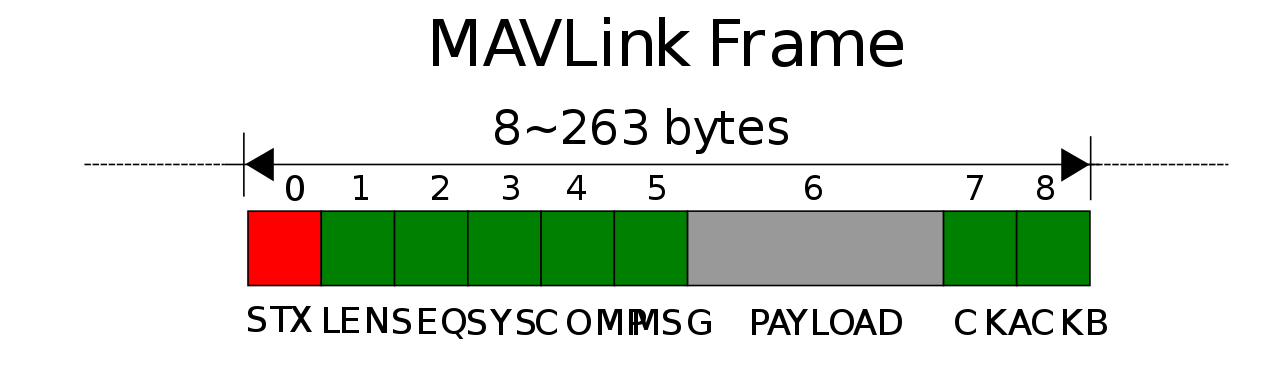
\includegraphics[width=0.7\linewidth]{./pics/mavlink}
	\caption{Структура пакет MAVLink
	}
	\label{fig:mavlink} % эта метка позволяет ссылаться на рисунок в тексте
\end{figure}

uint8\_t magic;              //Метка начала

uint8\_t len;                //Размер данных / длина полезной нагрузки (сообщения)

uint8\_t incompat\_flags;     //Обратно несовместимые флаги

uint8\_t compat\_flags;       //Обратно совместимые флаги

uint8\_t seq;                //Порядковый номер сообщения для выявления потери сообщения

uint8\_t sysid;              //ID системы-отправителя

uint8\_t compid;             //ID компонента-отправителя

uint8\_t msgid 0:7;          //ID сообщения (первый байт), от него зависит, какие данные будут лежать в полезной нагрузке пакета

uint8\_t msgid 8:15;         //ID сообщения (второй байт)

uint8\_t msgid 16:23;        //ID сообщения (третий байт)

uint8\_t payload[max 255];   //Полезная нагрузка (размер сообщения максимум 255 байт) 

uint16\_t checksum;          //Контрольная сумма

uint8\_t signature[13];      //Сигнатура (опционально)

Структура пакета MAVLink v1 аналогична, но опускает incompat\_flags, compat\_flags и signature, и имеет только один байт для адреса сообщения \cite{mavlink}.

%https://mavlink.io/en/about/overview.html
\subsubsection{Публикация}
Беспроводной формат MAVLink оптимизирован для систем с ограниченными ресурсами и, следовательно, порядок полей не такой, как в спецификации XML. Все поля сообщения сортируются по размеру, сначала с самыми большими полями (uint64\_t), а затем с меньшими полями. Сортировка выполняется с использованием стабильного алгоритма сортировки, который гарантирует, что любые поля, которые не нужно переупорядочивать, останутся в том же порядке. Это предотвращает проблемы с выравниванием в системах кодирования / декодирования и позволяет очень эффективно упаковывать / распаковывать данные \cite{mavlink}.

Примеры MAV\-Link-сообщений:

ATTITUDE, ATTITUDE\_QUATERNION – ориентация квадрокоптера в пространстве;

LOCAL\_POSITION\_NED – локальная позиция квадрокоптера;

GLOBAL\_POSITION\_INT – глобальная позиция квадрокоптера (широта / долгота / высота);

COMMAND\_LONG – команда для квадрокоптера (взлететь, сесть, переключить режим и т. д.) \cite{clover}.

\subsubsection{Многоадресные потоки и гарантированная доставка}
MAVLink создан для систем, в которых высокоскоростные потоки данных от беспилотников поступают в наземные станции, но смешиваются с передачами, требующими гарантированной доставки. Ключевой момент состоит в том, что для большинства потоков телеметрии не существует известного или единственного получателя: вместо этого, как правило, наземная станция управления нуждаются в одном и том же потоке данных.
С другой стороны, настройка бортовой миссии или изменение конфигурации системы с бортовыми параметрами требует точка -- точка связи с гарантированной доставкой. MAVLink достигает очень высокой эффективности за счет использования обоих режимов работы.

\subsubsection{Соединение точка -- точка}
В режиме точка -- точка при изменении миссии, параметры и передаче команд MAV\-Link использует идентификатор цели и целевой компонент \cite{mavlink}.

\subsubsection{Режим топиков (публикация -- подписка)}
В режиме топиков протокол не будет выдавать идентификатор целевой системы и компонента для сообщений, чтобы сэкономить пропускную способность канала. Типичными примерами этого режима связи являются все потоки данных автопилота, такие как положение, координаты и т. д \cite{mavlink}.

Основное преимущество этого режима заключается в том, что не создаются дополнительные накладные расходы, и все подписчики могут получать эти данные.

MAVLINK полезен тем, что позволяет получать практически всю информации о внутреннем состоянии полетного контроллера.
% дописать

\subsection{Robotic Operating System}
%\url{https://www.ros.org/about-ros/}

Robotic Operating System (далее ROS) -- это гибкая платформа для написания программного обеспечения для роботов; набор инструментов, библиотек и соглашений, которые призваны упростить задачу создания сложного и надежного поведения роботов на самых разных роботизированных платформах \cite{ros}.

Целью создания ROS является создание среды разработки, которая позволяет разработчикам ПО для роботов взаимодействовать на глобальном уровне.

ROS сосредоточена на максимизации повторного использования кода при разработке. Основные характеристики, позволяющие это реализовать:

1. Распределенные процессы. Структура ROS создана в виде минимальных единиц исполняемых процессов (нод), и каждый процесс выполняется изолированно. Взаимодействие разных нод происходит только на уровне обмена сообщениями.

2. Управление пакетами. Несколько процессов, имеющих общую задачу, объединяются в пакеты. Управление пакетами подразумевает набор утилит, позволяющих автоматически скачивать, устанавливать и удалять пакеты. Пакетный менеджер гарантирует работоспособность и целостность установленных пакетов.

3. Публичные репозитории и документация. Каждый доступный пакет хранится в публичном репозитории. Документация пакетов публикуется в единой системе, которая упрощает поиск необходимых пакетов.

4. Поддержка различных языков программирования. ROS предоставляет клиентские библиотеки для поддержки различных языков программирования. Наиболее популярны Python, C ++, а также такие языки, как Lisp, JAVA, C\#, Lua и Ruby \cite{voltbro}.

Для понимания устройства ROS необходимо ознакомиться с концепциями: ноды, топики, сервисы.

\subsubsection{Пакеты}
Программное обеспечение в ROS организовано в виде пакетов. Пакет может содержать ноды ROS, независимую от ROS библиотеку, набор данных, файлы конфигурации, стороннее программное обеспечение или что-либо еще, что логически составляет полезный модуль. Цель пакетов -- обеспечить доступ к перечисленным сущностям простым в использовании способом. В целом, пакеты ROS следуют принципу «Goldilocks»: достаточно функциональных возможностей, чтобы быть полезными, но не слишком много, чтобы пакет не был тяжелым и трудным для использования из другого программного обеспечения.

Пакеты можно создавать вручную или с помощью таких инструментов, как catkin\_create\_pkg . Пакет ROS -- это просто каталог, производный от ROS\_PACKAGE\_PATH, в котором есть файл package.xml, содержащий информацию о пакете. Пакеты -- это самая атомарная единица сборки и релиза. Это означает, что пакет -- это наименьшая отдельная сущность, которую можно создать в ROS, и это способ, которым программное обеспечение объединяется для релиза.
% http://wiki.ros.org/Packages

\subsubsection{Ноды}
Нода представляет собой процесс, который выполняет вычисления. Ноды объединяются в граф и взаимодействуют друг с другом с помощью топиков, сервисов и сервера параметров. Ноды предназначены для работы в мелком масштабе; система управления роботом обычно состоит из множества нод.

Ноды можно установить из публичных репозиториев, предоставляемых менеджером apt, или собрать вручную с помощью catkin\_make.
% дописано
Все ноды в графе имеют собственное имя, которое однозначно идентифицирует их для остальной системы. Самая старшая по иерархии нода зовется мастер-нодой. Ноды также имеют типы, которые упрощают процесс обращения к исполняемому файлу ноды в файловой системе. Эти типы представляют собой имена ресурсов пакета с именем пакета ноды и именем исполняемого файла ноды. Чтобы определить тип ноды, ROS ищет все исполняемые файлы в пакете с указанным именем и выбирает первый из найденных \cite{ros}. 
% http://wiki.ros.org/Nodes 

Очень многие робототехнические библиотеки и драйвера выполнены в виде ROS-нод.
Для того, чтобы преобразовать обычную программу в ROS-ноду, необходимо подключить к ней библиотеку rospy или roscpp и добавить инициализирующий код.

Пример ROS-ноды на языке Python представлен в листинге \ref{lst:1}:

\begin{Program}[H]
	\caption{Пример ROS-ноды на языке Python} \label{lst:1}
\begin{MyCode}
import rospy

rospy.init_node('my_ros_node')  # имя ROS-ноды

rospy.spin()  # входим в бесконечный цикл...
\end{MyCode}
\end{Program}

Возможность запуска нескольких нод в одном процессе осуществляет пакет nodelet. Он позволяет производить обмен сообщений внутри процесса без затрат на копирование \cite{ros}.

Для прямого запуска ноды из пакета используется утилита rosrun в следующем виде: \(\$ rosrun [ИмяПакета] [ИмяУзла]\).
%http://wiki.ros.org/nodelet

\subsubsection{Топики}
Топиками называют шины данных, по которым ноды обмениваются сообщениями. Топики имеют семантику анонимной публикации / подписки, которая отделяет издателей от их подписчиков. Как правило, ноды не знают, с кем они общаются. Вместо этого ноды, которые заинтересованы в данных, подписываются на соответствующие топики; ноды публикуют данные в топике. У топиков может быть несколько издателей и подписчиков.

Топики предназначены для однонаправленного потокового общения.

Каждый топик строго типизирован в соответствии с типом сообщения ROS, используемым для публикации в ней, и ноды могут получать сообщения только с совпадающим типом. Мастер-нода не обеспечивает согласованность типа среди издателей, и подписчики не будут устанавливать соединение, если топики не совпадают. Кроме того, все клиенты ROS проверяют совпадение хэш-индекса MD5, вычисленного из файлов msg с описанием сообщений. Эта проверка гарантирует, что ноды ROS были скомпилированы из публичных репозиториев \cite{ros}. Пример публикации сообщения в топик на языке Python приведен в листинге \ref{lst:2}:
% http://wiki.ros.org/Topics
%дописано
\begin{Program}[H]
	\caption{Пример публикации сообщения типа std\_msgs / String (строка) в топик foo} \label{lst:2}
\begin{MyCode}
from std_msgs.msg import String

# создаем Publisher'а
foo_pub = rospy.Publisher('/foo', String, queue_size=1)

# публикуем сообщение
foo_pub.publish(data='Hello, world!')
\end{MyCode}
\end{Program}

\begin{Program}[H]
	\caption{Пример подписки на топик /foo на языке Python} \label{lst:3}
\begin{MyCode}
def foo_callback(msg):
	print msg.data

#При получении сообщения в топик /foo
#будет вызвана функция foo_callback.
rospy.Subscriber('/foo', String, foo_callback)
\end{MyCode}
\end{Program}

Также существует возможность работы с топиками с помощью утилиты rostopic. Например, с помощью следующей команды можно просматривать сообщения, публикуемые в топик /mavros/state:

\$ rostopic echo /mavros/state
\subsubsection{Сервисы}

Сервис -- это некоторый аналог функции, которая может быть вызвана из одной ноды, а обработана в другой. У сервиса есть имя, аналогичное имени топика, и 2 типа сообщений: тип запроса и тип ответа \cite{clover}. Пример вызова ROS-сервиса из языка Python приведен в листинге \ref{lst:4}:

\begin{Program}[H]
	\caption{Пример вызова ROS-сервиса из языка Python} \label{lst:4}
\begin{MyCode}
from clover.srv import GetTelemetry

# Создаем обертку над сервисом get_telemetry
# пакета clover с типом GetTelemetry:
get_telemetry = rospy.ServiceProxy('get_telemetry',
srv.GetTelemetry)

# Вызываем сервис и получаем телеметрию квадрокоптера:
telemetry = get_telemetry()
# С сервисами можно также работать при помощи утилиты rosservice.
# Так можно вызвать сервис /get_telemetry из командной строки:

rosservice call /get_telemetry "{frame_id: ''}"
\end{MyCode}
\end{Program}

\subsubsection{Запуск ROS}
Запуск ROS среды производится запуском roscore. Это необходимо, чтобы ноды могли обмениваться данными \cite{pkg}.

roscore -- это набор нод и программ, которые являются предпосылками системы на основе ROS \cite{ros}. Запускается с помощью команды \(\$ roscore\) в одной из вкладок консоли, однако при использовании roslaunch это действие необязательно -- при выполнении roslaunch первым делом запускается roscore.

roslaunch -- это инструмент для простого запуска нескольких нод ROS. Он включает в себя опции для автоматического запуска уже завершенных процессов. roslaunch принимает один или несколько файлов конфигурации XML (с расширением .launch), определяющих параметры, которые необходимо установить, и ноды для запуска, а также машины, на которых они должны запускаться \cite{ros}.

\subsubsection{MAVROS}
%\url{https://clover.coex.tech/ru/mavros.html}
%\url{https://dev.px4.io/master/en/ros/mavros\_installation.html}
Так как выбран ROS как основной фреймворк для реализации проекта и MAVLink, в качестве основного протокола -- необходим компонент, обеспечивающий взаимодействие обозначенных систем.
MAVROS (MAVLink + ROS) -- это пакет для ROS, предоставляющий возможность общаться с беспилотниками по протоколу MAVLink. MAVROS поддерживает полетные стеки PX4 и APM. Связь организовывается по UART, USB, TCP или UDP.

%MAVROS как нода подписывается на ROS-топики в ожидании команд, публикует в другие топики телеметрию, и предоставляет сервисы.
% дописано
Пакет mavros обеспечивает расширяемую связь MAVLink между компьютерами, на которых работают ROS, автопилоты с поддержкой MAVLink и GCS с поддержкой MAVLink. Нода MAVROS запускается в launch-файле \cite{clover}.
launch-файл содержит следующие параметры:
\begin{itemize}
\item  system\_id (INT, значение по умолчанию: 1) -- cистемный идентификатор узла MAVLink;

\item  component\_id (INT, по умолчанию: 240) -- ID компонента узла MAVLink;

\item  target\_system\_id (INT, значение по умолчанию: 1) -- системный идентификатор FCU MAVLink;

\item  target\_component\_id (INT, значение по умолчанию: 1) -- идентификатор компонента FCU MAVLink;

\item  startup\_px4\_usb\_quirk (bool, по умолчанию: false) -- определение, применить quirk для PX4 или нет;

\item  plugin\_blacklist (string[], по умолчанию: []) -- черный список псевдонимов (глобальный синтаксис, пример: ['rc *']);

\item  plugin\_whitelist (string[], по умолчанию: []) -- белый список псевдонимов (глобальный синтаксис, отменяет черный список);

\item  fcu\_url (string, по умолчанию: / dev / ttyACM0: 57600) -- URL-адрес подключения FCU;

\item  fcu\_protocol (string, по умолчанию: v2.0) -- версия протокола MAVLink;

\item  gcs\_url (string, по умолчанию: udp) -- URL-адрес GCS \cite{ros}.
\end{itemize}
% дописано

\subsection{Компьютерное зрение}
%дописано для чего нужно (основная задача получать вижуал поз)+ вступление про опенсв
Одна из главных задач работы заключается в навигации дрона в пространстве, не основываясь на показаниях датчиков подобных лазерному дальномеру и барометру, поскольку в миниатюрных размерах они имеют большую погрешность. Ориентиром в данной ситуации может стать видеопоток с бортовой камеры. Распознавая контуры объектов в кадре и соотнося их с реальными размерами возможно получение координат дрона в локальной системе. Посулярным инструментом для распознавания является OpenCV (Open Source Computer Vision Library) -- это библиотека с открытым исходным кодом, которая включает в себя несколько сотен алгоритмов компьютерного зрения. Она реализована на C/C++, также разрабатывается для Python, Java и других языках, а распространяется в условиях лицензии BSD \cite{opencv}.

В ходе изучения стандартных способов распознавания объектов в OpenCV был найден такой ориентир как навигационные метки под названием ArUco. Рассмотрим подробнее их структуру.

\subsubsection{ArUco маркеры}

Для позиционирования робототехнических систем с помощью компьютерного зрения используются ArUco маркеры -- квадратные маркеры, состоящие из широкой черной границы и внутренней двоичной матрицы, которая определяет его идентификатор (id). Черная рамка облегчает ее быстрое обнаружение на изображении, а двоичная кодификация позволяет ее идентифицировать \cite{opencv}.

Первое сообщение о маркерах ArUco появилось в 2014 году в работе S.Garrido-Jurado с соавторами «Automatic generation and detection of highly reliable fiducial markers under occlusion», что на русском звучит как «Автоматическая генерация и высоконадежное обнаружение фидуциальных маркеров при окклюзии».
Окклюзия (англ. occlusion от лат. occlusio «сокрытие») — термин, который указывает на какое-либо состояние, которое обычно открыто, а в определённый момент времени полностью закрыто.
Фидуциальный маркер или фидуциал — это объект, помещенный в поле зрения системы визуализации, который появляется в полученном изображении, для использования в качестве точки отсчета или меры. Это может быть либо что-то, помещенное в / или на предмет изображения, либо метка или набор меток в сетке оптического прибора.
ArUco расшифровывается как Augmented Reality University of Cordoba (Университет дополненной реальности в Кордове) \cite{aruco}.
% дописано

Размещая маркеры на доске и прописывая их реальные размеры и последовательность, получаем возможность использовать углы всех маркеров для оценки положения камеры по отношению ко всей доске.
Используя набор независимых маркеров, можно оценить позу для каждого маркера индивидуально, так как неизвестно относительное положение маркеров в окружающей среде.

Основные преимущества использования доски (рисунок \ref{fig:aruc}):
\begin{itemize}
\item оценка позы намного более универсальна; для оценки позы необходимы только некоторые маркеры, а значит, позу можно рассчитать даже при наличии окклюзии или частичных видов;
\item полученная поза обычно более точна, поскольку используется большее количество точечных соответствий (углов маркеров).
\end{itemize}
%https://docs.opencv.org/master/db/da9/tutorial_aruco_board_detection.html
% ~\ref{fig:aruc}
\begin{figure}[H]
	\centering
	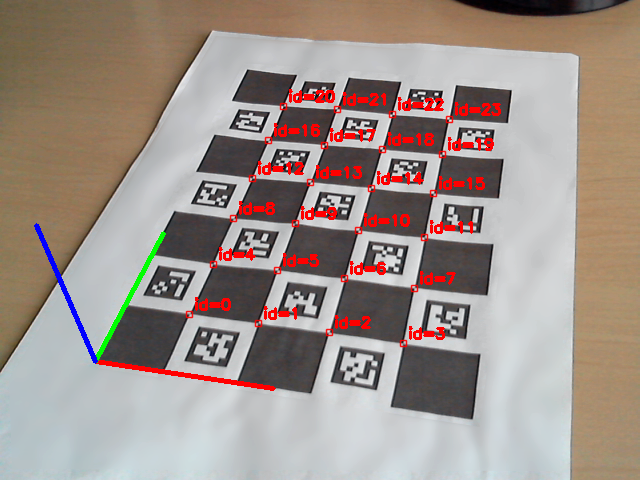
\includegraphics[width=0.5\linewidth]{pics/aruc}
	\caption{Пример распознанной доски с маркерами
	}
	\label{fig:aruc}
\end{figure}
%https://docs.opencv.org/3.1.0/d5/dae/tutorial_aruco_detection.html

Каждый обнаруженный маркер включает:
\begin{itemize}
\item положение его четырех углов на изображении (в исходном порядке);
\item идентификатор маркера.
\end{itemize}

Процесс обнаружения маркера состоит из двух основных этапов:

1. Обнаружение кандидатов в маркеры. На этом этапе изображение анализируется, чтобы найти квадратные формы, которые могут быть маркерами. Процесс начинается с адаптивного определения порога для сегментации маркеров, затем контуры извлекаются из изображения с пороговым значением, а те, которые не являются выпуклыми или не приближаются к квадратной форме, отбрасываются. Также применяется некоторая дополнительная фильтрация (удаление слишком мелких или слишком больших контуров, удаление контуров слишком близко друг к другу и т. д.).

2. После обнаружения кандидатов необходимо определить, действительно ли они являются маркерами, путем анализа их внутренней кодификации. Этот шаг начинается с извлечения маркерных битов каждого маркера. Для этого сначала применяется перспективное преобразование для получения маркера в его канонической форме. Затем каноническое изображение определяется с помощью метода Оцу (алгоритм вычисления порога бинаризации для полутонового изображения) для разделения белых и черных битов. Изображение делится на разные ячейки в соответствии с размером маркера и размером границы, а количество черных или белых пикселей в каждой ячейке подсчитывается, чтобы определить, является ли это белым или черным битом. Наконец, биты анализируются, чтобы определить, принадлежит ли маркер определенному словарю, и при необходимости используются методы исправления ошибок \cite{opencv}.

\subsection{Потоковая передача видео}
\subsubsection{GStreamer}

GStreamer -- это библиотека для построения компонентов обработки мультимедиа. 
% дописать 
Он поддерживается различными мультимедийными приложениями, позволяет осуществлять потоковую передачу аудио / видео и обрабатывать звук / видео. GStreamer является свободным программным обеспечением с лицензией GNU LGPL.

Практически все в GStreamer является элементом. Все, начиная от обычных источников потоков (filesrc, alsasrc, и т. п.), обработчиков потоков (декодеры, фильтры, и т. п.) и заканчивая конечными устройствами вывода (alsasink, fakesink, filesink, и т. п.).

Pad -- это некая точка подключения одного элемента к другому, если более просто -- это входы и выходы элемента (рисунок \ref{fig:ris12}). Обычно они именуются «sink» -- вход и «src» -- выход.
% ~\ref{fig:ris1}
\begin{figure}[H]
	\centering
	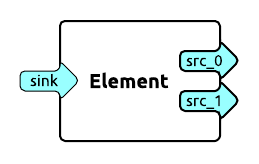
\includegraphics[width=0.5\linewidth]{pics/pic1}
	\caption{ GStreamer pads (sink, src\_0, src\_1)
	}
	\label{fig:ris12}
\end{figure}

Жизненный цикл элементы проводят внутри контейнеров. Контейнер управляет рассылкой сообщений от элемента к элементу, статусами элементов. Контейнеры делятся на два вида: Bin и Pipeline.

Bin -- простой контейнер, который управляет рассылкой сообщений от элемента к элементу которые находятся внутри него. Bin обычно используется для создания группы элементов которые должны совершать какое-либо действие. 
Pipeline является контейнером верхнего уровня, он управляет синхронизацией элементов, рассылает статусы. Например, если pipeline установить статус PAUSED, этот статус будет автоматически разослан всем элементам которые находятся внутри него. Pipeline является реализацией Bin \cite{gstreamer}. 

Источники данных -- это класс плагинов GStreamer, который позволяет читать медиаданные из различных источников, таких как файловая система или аудио-входы звуковой карты. Также, они позволяют получать медиапоток с различных серверов потокового вещания, таких как HTTP (ICECast, ShoutCast), RTSP, RTMP, TCP и UDP. 

Утилита gst-launch-1.0 позволяет запускать GStreamer pipeline без написания кода. Запуск pipeline имеет следующий вид:
gst-launch-1.0 описание-pipeline

Описание pipeline, в свою очередь, делится на описание элементов вида:
element1 property1=value1 property2=value2 ! element2.

Есть элемент типа element1 со свойствами property1 и property2, которые имеют значения value1 и value2 соответственно, и есть элемент типа element2. Символ «!» указывает на то, что выход element1 необходимо соединить с входом element2.
%https://habr.com/ru/post/179167/
% https://docs.gstreamer.com/documentation/
Для приема и обработки видеопотока на наземной станции может быть использован gscam.

\subsubsection{gscam}
gscam -- ROS нода, представляющая собой драйвер. gscam может быть запущен и как нода, и как нодлет.
Для запуска gscam необходимо определить переменную окружения GSCAM\_CONFIG, которую будет использовать gstreamer для получения трансляции.
% дописано

gscam получает трансляцию и публикует 2 топика: /camera/image\_raw (необработанное изображение) и /camera/camera\_info (содержит калибровку камеры и дополнительные данные о конфигурации камеры) \cite{ros}.
% http://wiki.ros.org/gscam

\subsubsection{aruco\_gridboard}
Нода aruco\_gridboard подписывается на топики, публикуемые gscam. При получении видеопотока aruco\_gridboard распознает карту aruco маркеров, описанную в файле yaml, рассчитывает координаты относительно карты, и публикует статус в топик /vision/status, а полученные координаты в /vision/pose. Файл yaml содержит коэффициент масштаба маркеров на изображении, координаты углов каждого маркера и их идентификационные номера.

Таким образом, видео с Raspberry Pi c помощью gstreamer передается на ip-адрес наземной станции; нода gscam получает пакеты и публикует изображение в топики /camera/image\_raw и /camera/camera\_info; aruco\_gridboard подписывается на топики с изображением и информацией о камере и публикует сообщения о положении дрона относительно карты маркеров в /mavros/vision\_pose/pose топик.

%http://www.uco.es/investiga/grupos/ava/sites/default/files/GarridoJurado2014.pdf

